\subsection*{Реплицированные объекты. Заполнение областей}
\addcontentsline{toc}{subsection}{Реплицированные объекты. Заполнение областей}

\textbf{Задание:}\\
Научиться работать с объектами презентации и элементами управления.\\

\textbf{Решение:}\\
В среде AnyLogic существуют такие элементы презентации как области просмотра, они предназначены для упрощения демонстрации объектов, находящихся на достаточно больших расстояниях друг от друга. Для осуществления перехода между областями просмотра можно использовать как блоки элементов управления, такие как кнопки и обычные элементы презентации, например текст. (Рисунок \ref{fig:moving_rectangle1})
\begin{figure}[h]
	\centering 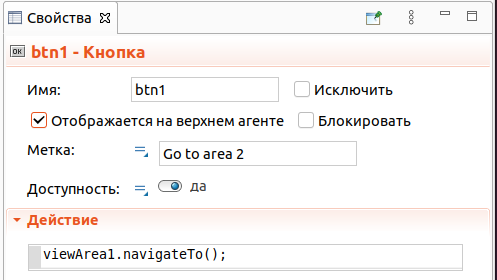
\includegraphics[scale=0.3]{replications1}
	\caption{Переход между областями просмотра}
	\label{fig:replications1}
\end{figure}

Иногда перед пользователем стоит задача создания некого количества равноудаленных друг от друга одинаковых элементов, в этом случае он может воспользоваться такими свойствам элементов презентации как указание количества элементов и их координат, зависящих от индекса. (Рисунок \ref{fig:replications2})
\begin{figure}[h]
	\centering 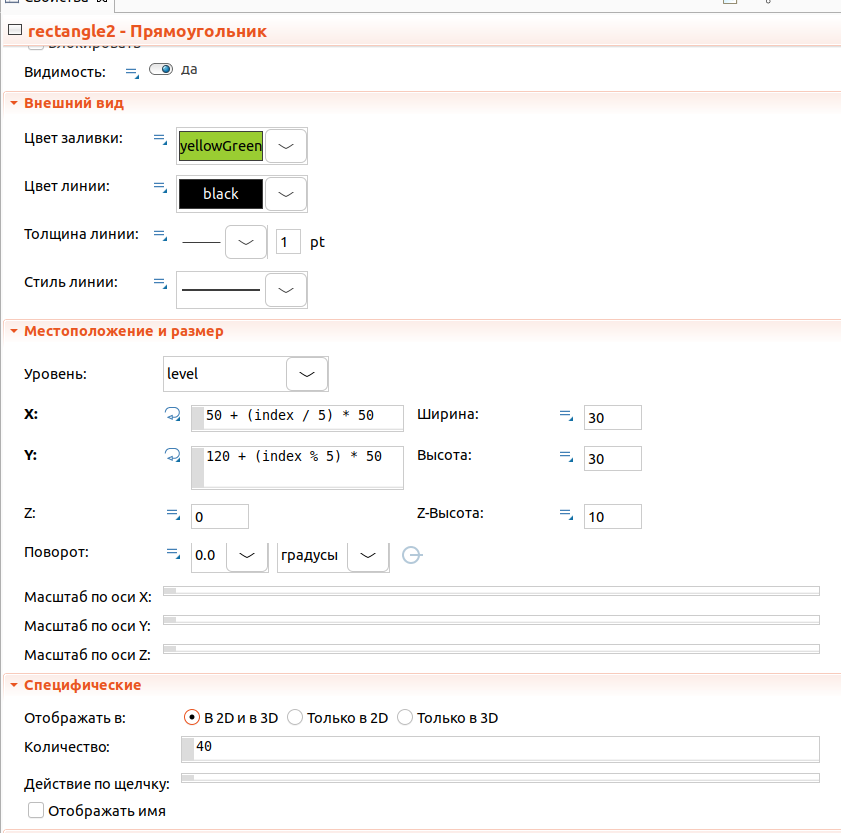
\includegraphics[scale=0.25]{replications2}
	\caption{Задание количества и местоположения элементов}
	\label{fig:replications2}
\end{figure}

\begin{figure}[h]
	\centering 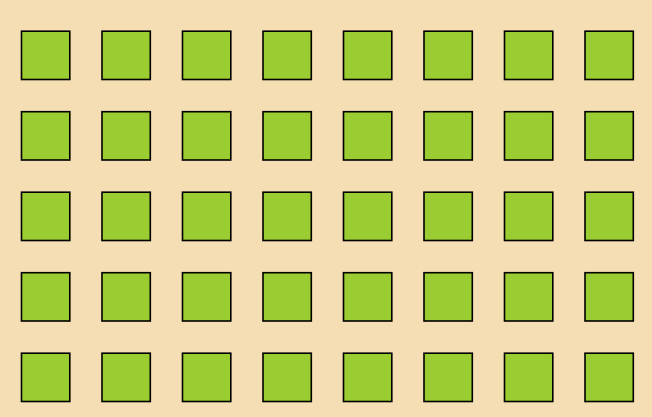
\includegraphics[scale=0.4]{replications3}
	\caption{Вид заданных элементов при демонстрации}
	\label{fig:replications3}
\end{figure}

Положение реплицированных элементов можно так же менять с течением времени. (Рисунок \ref{fig:replications4})

\begin{figure}[h]
	\centering 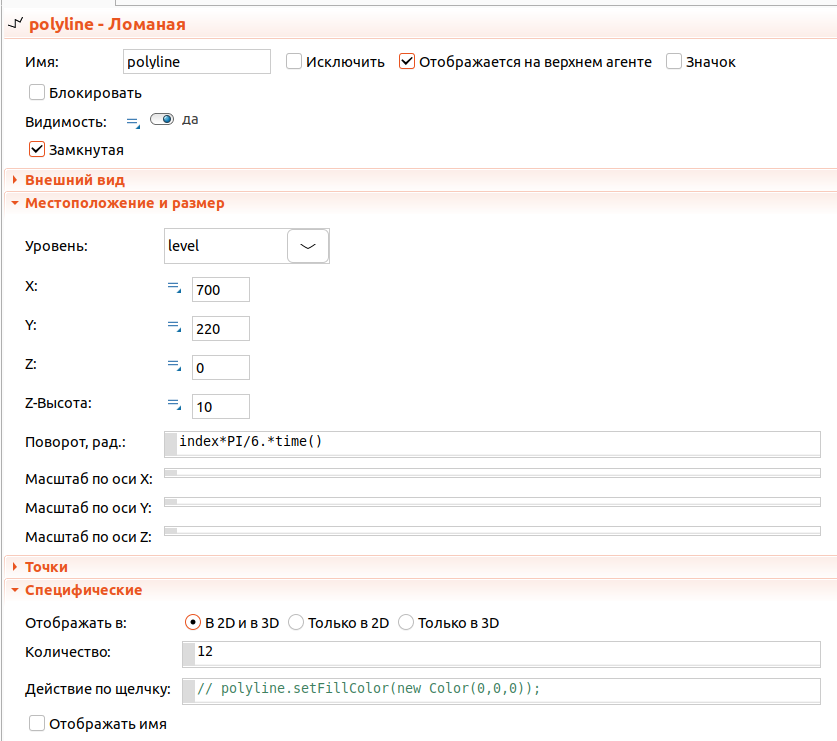
\includegraphics[scale=0.3]{replications4}
	\caption{Изменение положения элементов в зависимости от времени}
	\label{fig:replications4}
\end{figure}

\newpage

\begin{figure}[h]
	\centering 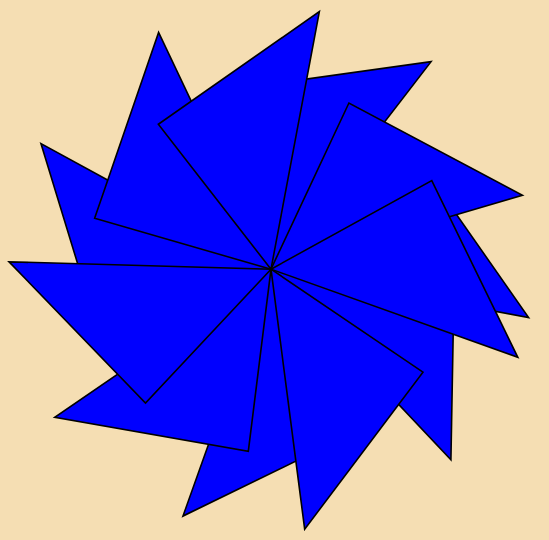
\includegraphics[scale=0.3]{replications5}
	\caption{Вид заданных элементов при демонстрации}
	\label{fig:replications5}
\end{figure}

Таким образом, нами были изучены основные механики работы с объектами презентации и элементами управления.